%%%%%%%%%%%%%%%%%%%%%%%%%%%%%%%%%%%%%%
\section{Background} \label{background}
%%%%%%%%%%%%%%%%%%%%%%%%%%%%%%%%%%%%%%
% \begin{figure}
%     \centering
%     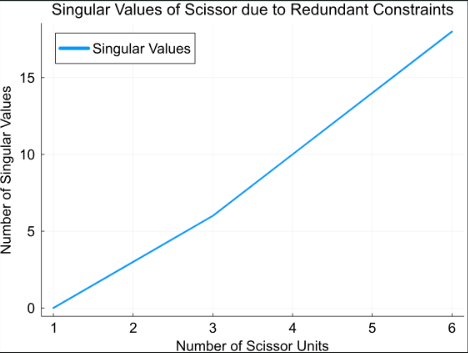
\includegraphics[width=\linewidth]{DOJO-CCK/Figures/singular_values_scissor.png}
%     \caption{The growth of singular values for scissor mechanism}
%     \label{fig:singular-vals}
% \end{figure}
% \includegraphics[width=\linewidth]{example-image-a}
This section briefly reviews multi-body dynamics with constraints and the singular-value decomposition (SVD).

\subsection{Dynamics} We leverage a differentiable physics engine, Dojo \cite{howell_dojo_2022}, which is based on “maximal coordinates,” in which each link is parameterized by its full SE(3) pose, and joints are represented with explicit constraints. The maximal-coordinate dynamics are described by:
\begin{equation}
\textbf{x} = \begin{bmatrix}
    \textbf{x}_1 \\
    \vdots \\
    \textbf{x}_n
\end{bmatrix}, \ \textbf{x}_i = \begin{bmatrix}
    \textbf{r}_i \\ \textbf{q}_i \\ \textbf{v}_i \\ \boldsymbol{\omega}_i
\end{bmatrix},    \dot{\textbf{x}} = \begin{bmatrix}
    \dot{\textbf{x}}_1 \\ 
    \vdots \\ 
    \dot{\textbf{x}}_n
\end{bmatrix}
% \label{eq:space_struct1}
\end{equation}
\begin{equation}
    \dot{\textbf{x}}_i = \begin{bmatrix}
    {\textbf{v}}_i \\ \frac{1}{2}\textbf{q}_i \otimes \boldsymbol{\omega}_i \\ M_i^{-1} \cdot (\textbf{f}_{\text{ext}, i} + \textbf{f}_{\text{int}, i}) \\ J_i^{-1} \cdot (\boldsymbol{\tau}_{\text{ext}, i} + \boldsymbol{\tau}_{\text{int}, i} - \boldsymbol{\omega}_i \times J_i \cdot \boldsymbol{\omega}_i)
\end{bmatrix}  
\end{equation}
\begin{equation}
    \begin{bmatrix}
    \textbf{f}_{int} \\
    \boldsymbol{\tau}_{int}
\end{bmatrix}  = \frac{\delta c(\textbf{x})}{\delta \textbf{x}}^T\boldsymbol{\lambda}
\end{equation}
% \begin{equation}
%      \textbf{f}_{\text{ext}, i} = \textbf{u}_{f,i} + M_i \cdot \textbf{g}, \quad \textbf{f}_{\text{int}, i} = -K_x \Delta \textbf{p}_{ij} - C_x \Delta \textbf{v}_{ij}
%      \label{eq:space_struct2}
% \end{equation}
% \begin{equation}
%     \boldsymbol{\tau}_{\text{ext}, i} = \textbf{u}_{\tau,i} + \textbf{p}_i \times \textbf{q}_i \otimes (\textbf{f}_{\text{ext}, i} + \textbf{f}_{\text{int}, i})
%     \label{eq:space_struct3}
% \end{equation}
% \begin{equation}
%     \boldsymbol{\tau}_{\text{int}, i} = -K_t \Delta \boldsymbol{\phi}_{ij} - C_t \Delta \boldsymbol{\omega}_{ij} 
% \end{equation}
where \(\textbf{r}_i \in {{\mathbb{R}}^3}\) represents the position vector for each body, \(\textbf{q}_i\in {{\mathbb{H}}}\) is the quaternion representing orientation of the body, \(\textbf{v}_i \in {{\mathbb{R}}^3}\) is the linear velocity, and \(\boldsymbol{\omega}_i \in {{\mathbb{R}}^3}\) is the angular velocity of each body. The mass matrix of a body is \(M_i\), and the inertia matrix is \(J_i\). Finally, the holonomic constraints, such as joints, are represented by $c(\textbf{x})$. The Lagrange multipliers $\boldsymbol{\lambda}$ represent the constraint forces and torques that satisfy these constraints. 

Representing a linkage mechanism using maximal coordinates offers several advantages: First, it avoids the challenges of defining generalized coordinates for closed kinematic chains, especially as linkage complexity grows. Second, using maximal coordinates makes representing joint clearances with inequality constraints straight forward. Finally, maximal coordinates provide direct correlations between joint-constraint values and the forces and torques acting on the body, offering clearer insight into the load distribution across linkage members. 

\subsection{Joint Constraints}
Incorporating joint constraints using Lagrange multipliers is a key technique in multibody dynamics, as it integrates constraints directly into the equations of motion. Lagrange multipliers introduce additional variables that represent the forces or torques necessary to enforce the joint conditions.
\begin{figure}
    \centering
    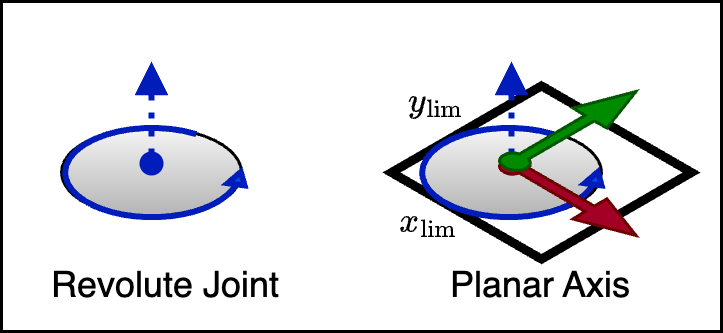
\includegraphics[width=0.8\linewidth]{Figures/joint_description.drawio.png}
    \caption{Diagrams of revolute and planar axis joint prototypes that are used to construct mechanism with clearance.}
    \label{fig:joint-proto}
\end{figure}
This work primarily deals with revolute joint-based mechanisms with joint clearance,  which is described using a planar-axis joint seen in Figure \ref{fig:joint-proto}. This joint allows the bodies to translate freely within a prescribed rectangular area with respect to each other. 

Although this approach is geometrically imprecise, the constraint typically positions the bodies near the corners of the rectangular constraint boundary, where the constraint forces are a linear combination of the adjacent sides. As a result, the force distribution closely resembles that of circular or elliptical constraints. The planar-axis joint was selected due to the current implementation in Dojo. Future work will explore more accurate joint constraints that better reflect the actual clearances in linkage mechanisms.

\subsection{Singular Value Decomposition}\label{sec:svd}
Singular Value Decomposition (SVD) is a powerful linear algebra technique widely used in model reduction to simplify complex systems while retaining essential dynamic features. SVD decomposes a matrix into three factors: 
\begin{equation}
    USV = \operatorname{SVD}(A)
\end{equation}
% \begin{equation}
%     A = USV^T
% \end{equation}
where $U$ is an orthogonal matrix of left singular vectors, $S$ is a diagonal matrix of singular values, and $V$ is an orthogonal matrix of right singular vectors. In the context of model reduction, SVD identifies the most significant modes of a system by ranking the singular values, which represent the importance or energy contribution of each mode. By truncating smaller singular values, we can create a reduced-order model that approximates the original system without the ill-conditioning from redundant, constrained degrees of freedom:
\begin{equation}
    \Tilde{A} = U[:, 1:r]S[1:r, 1:r]V[:,1:r]^T ,
\end{equation}
where $\Tilde{A}$ is the approximated rank-reduced matrix with rank $r$. Importantly for us, the SVD can factorize rectangular and rank-deficient matrices and is numerically robust.  

% This approach is particularly beneficial in large-scale linkage analysis, where computational efficiency is critical without sacrificing accuracy.

% Closed loop mechanisms suffer from numerical instability brought through redundant constraints. Our method systematically removes redundant constraints by using a singular value decomposition (SVD), resulting in a numerically robust method that takes steps only in the instantaneously unconstrained degrees of freedom of the system.
